\documentclass[12pt]{article}

\usepackage{pdflscape}
\usepackage[margin=0.8in]{geometry}
\usepackage{titling}
\usepackage{graphics} %Required for diagrams
\usepackage[hidelinks]{hyperref}
\usepackage{color}
\usepackage{framed}
\usepackage{epsfig}
\usepackage{epstopdf}

\begin{document}

\begin{titlepage}
	\begin{center}
		
		\begin{figure}[t]
			\centering
			
\includegraphics[width=350px]{images/UP_Logo.png}
		\end{figure}
		
		% Title
		\textsc{\large Project Tender} \\ 
		\vspace{2cm}
		\textbf{\Huge Project: RMB's Data Lake} \\ 
		\textsc{\large Client: RMB} \\ 
		\vspace{2cm}
		\textbf{\Huge Team: Team Name } \\ 
		
		%\begin{minipage}{0.4\textwidth}s
		\begin{flushright} \large
			Armand Pieterse \emph{u12167844} \newline
			Kgomotso Sito 		\emph{u12243273} \newline
			student name		\emph{uXXXXXXXX} \newline
			Sphelele Malo 	\emph{u12247040} \newline
			\end{flushright}
		%\end{minipage}
		\textsc{\small Department of Computer Science, University of Pretoria}
		
		\vfill
		
	Here's a link to \href{https://github.com/SpheMalo/COS-301-Main-Project.git}{GitHub}.\\
	\url{https://github.com/SpheMalo/COS-301-Main-Project.git}

	\vfill

	{\large \today}		
		
		
	\end{center}
\end{titlepage}


\newpage
\tableofcontents

\newpage
\listoffigures

\newpage

\section{Vision and scope}

\subsection{Project Background}

\subsection{Project vision}

\subsection{Project scope}

\newpage
\section{Application requirements and design}
\par{This section discusses for each module of the Figbook system the functional requirements
as well as the process designs for the use cases and the domain models which must be maintained
within persistent storage by that module.
}

\subsection{Authentication}

\subsubsection{scope}
\par{This section provides the details use case requirements for the use cases offered by the Authentication
module.}
\begin{figure}[h]
	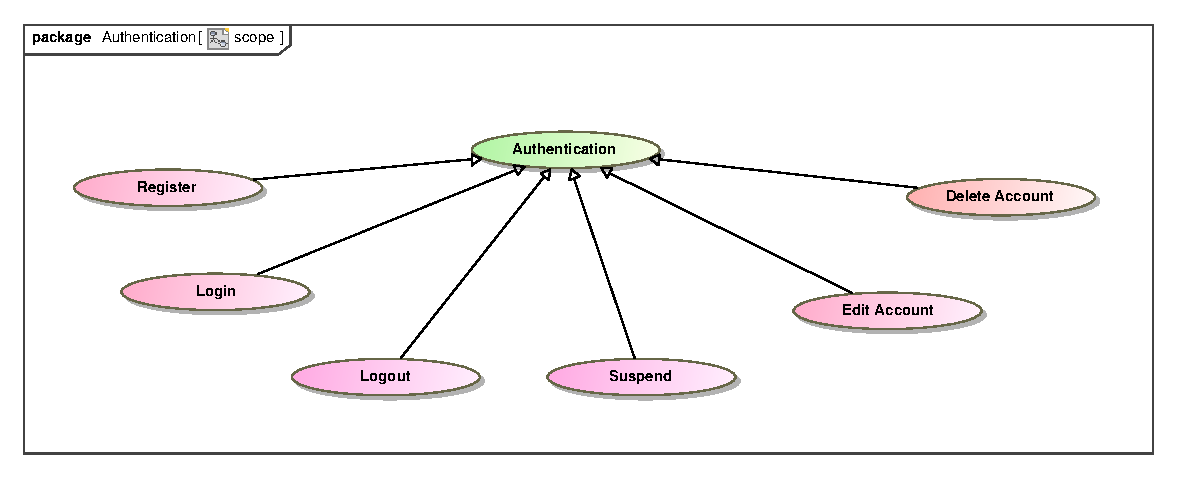
\includegraphics[height=200px, width=500px]{epsImages/Authentication/AuthenticationScope.eps}
	\caption{Scope for authentication module}
\end{figure}

\newpage
\subsubsection{Use Cases}

\begin{enumerate}


\item \textbf{registerAccount  – priority: critical } 
This use case creates  a user account and is persisted through to database.

\par{\textbf{service contract} The service contract for the registerAccount  service is shown in figure below. The pre-conditions are enforced (raising the appropriate exception should they not be met) and the requested account is created and persisted through to database.}
\begin{figure}[h]
		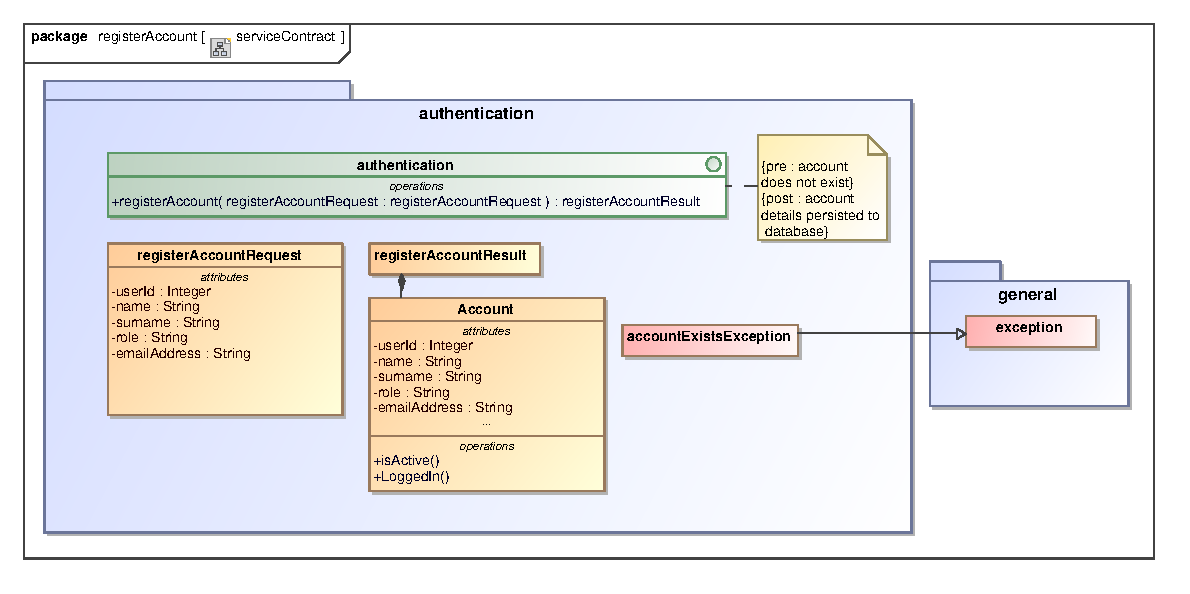
\includegraphics[height=200px, width=500px]{epsImages/Authentication/serviceContract.eps}
		\caption{Service contract for logging into a user account}
\end{figure}
\item \textbf{Login - priority: critical}
This use case allows a user to log into an existing account.

\par{\textbf{service contract} The service contract for the login service is shown in figure below.}
\begin{figure}[h]
		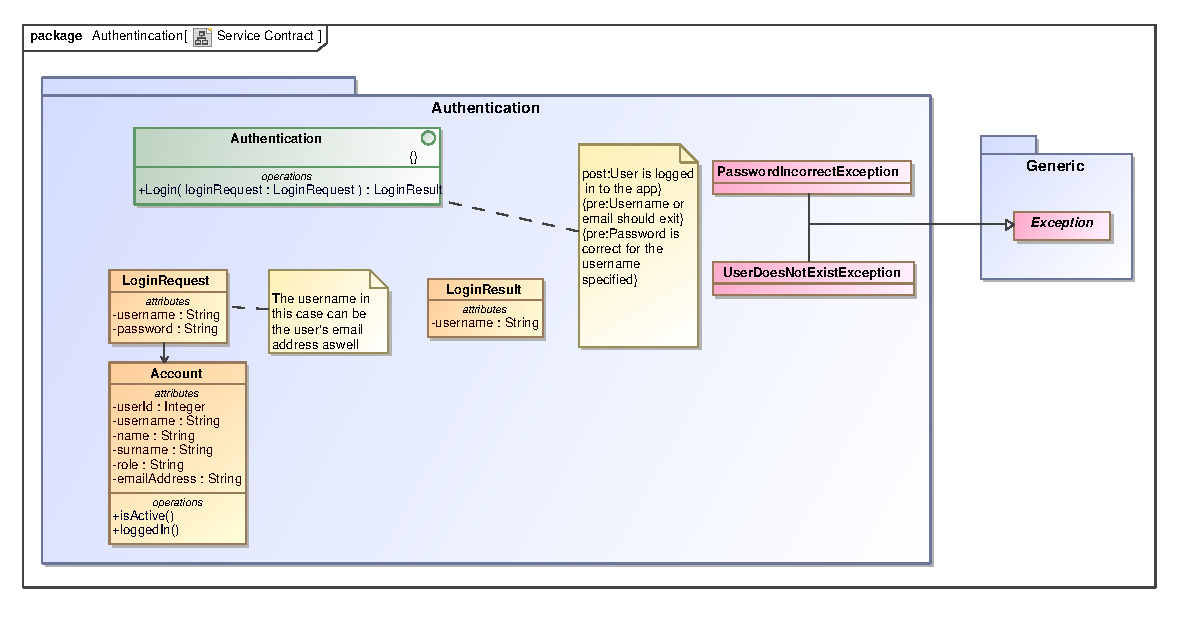
\includegraphics[height=200px, width=500px]{epsImages/Authentication/LoginServiceContract.eps}
		\caption{Service contract for logging into a user account}
\end{figure}

\item \textbf{Logout - priority: important} \\
This use case allows a user to log out of the system safely.

\par{\textbf{Service contract:} The service contract for logging out is shown below. The preconditions are enforced and the users session is ended, thus logging the user out of the system.}
\begin{figure}[h]

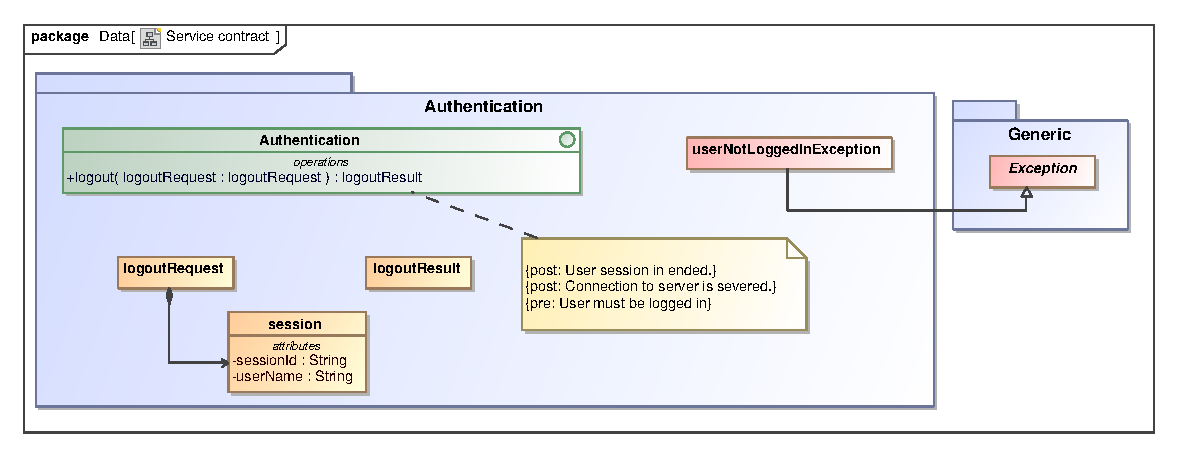
\includegraphics[scale=.9]{epsImages/Authentication/logoutServiceContract.eps}
\caption{Service contract for logging a user out of the system}
\end{figure}
\item \textbf{EditAccount}
\item \textbf{deleteAccount  – priority: important} 
This use case creates  a user account and is persisted through to database.

\par{\textbf{service contract} The service contract for the deleteAccount  service is shown in figure below. The pre-conditions are enforced (raising the appropriate exception should they not be met) and the account of interest is deleted and changes are persisted through to database.}

\begin{figure}[h]
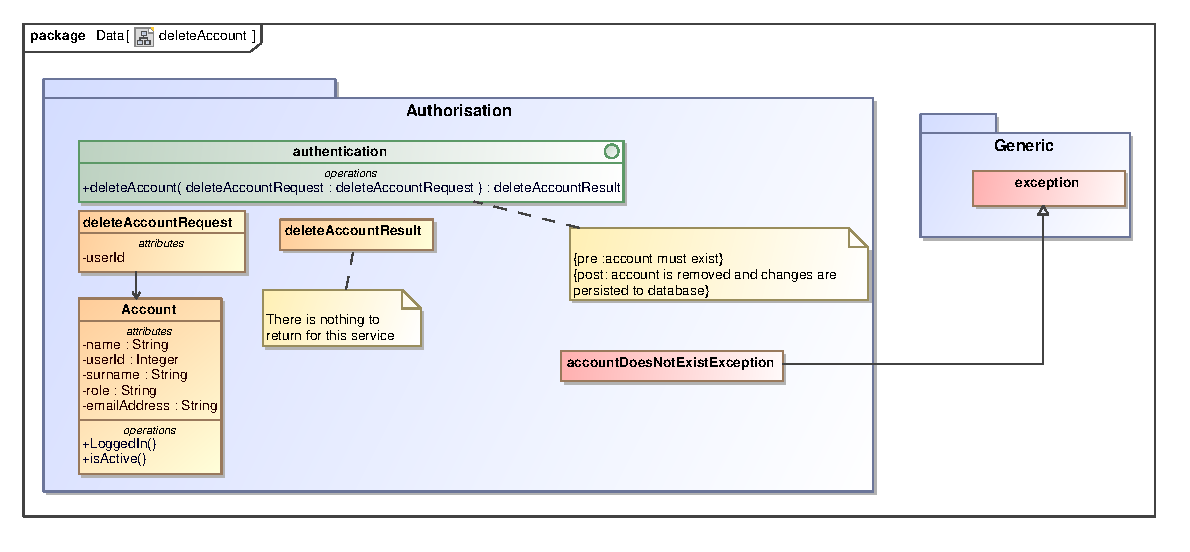
\includegraphics[height=200px, width=500px]{epsImages/Authentication/deleteAccount.eps}
\caption{Service contract for deleting a users account}
\end{figure}
\item \textbf{SuspendAccount - priority: important}\\
This use case allows the system administrator to suspend a users account for any reason he/she may see as appropriate. A suspended account bars the user from logging in and/or using the account until the administrator lifts the suspension.
\\ \textbf{service contract:} The service contract for the suspendAccount service is shown below. 
\begin{figure}[h]
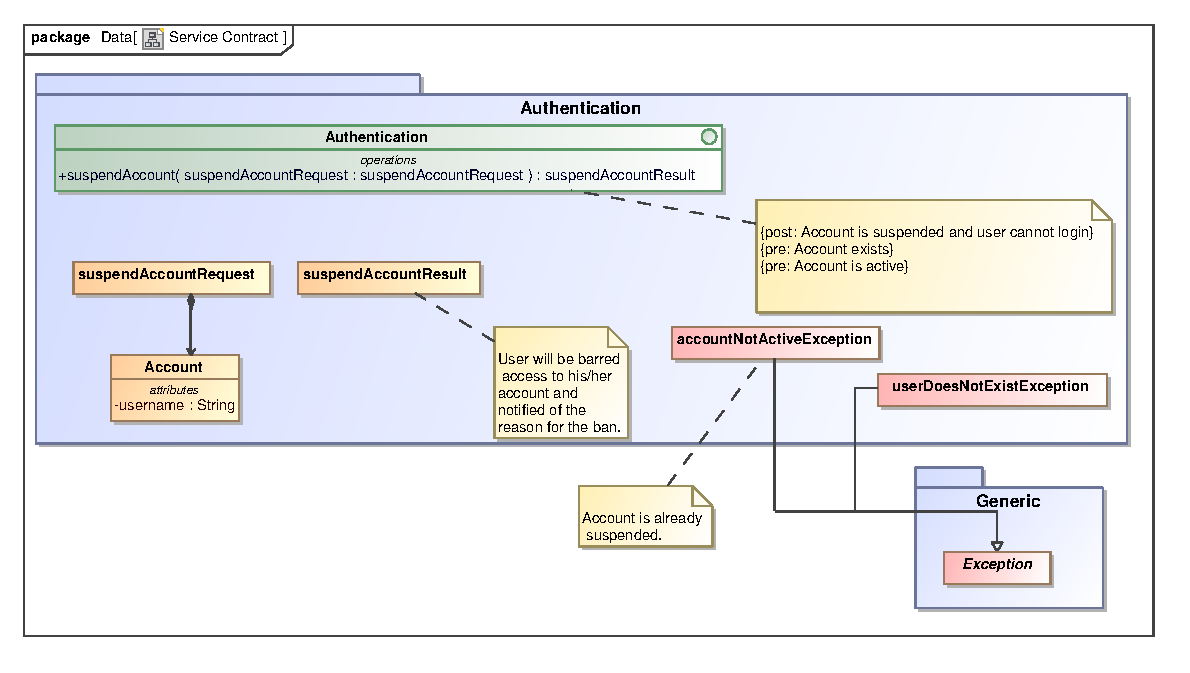
\includegraphics[height=250px, width=500px]{epsImages/Authentication/suspendServiceContract.eps}
\caption{Service contract for suspending a users account}
\end{figure} 
\end{enumerate}

\newpage
\subsection{Manuscript Management}

\subsubsection{scope}
\par{This section provides the detailed service contracts for the use cases offered by the Manuscript Management module.}

\begin{figure}[h]
	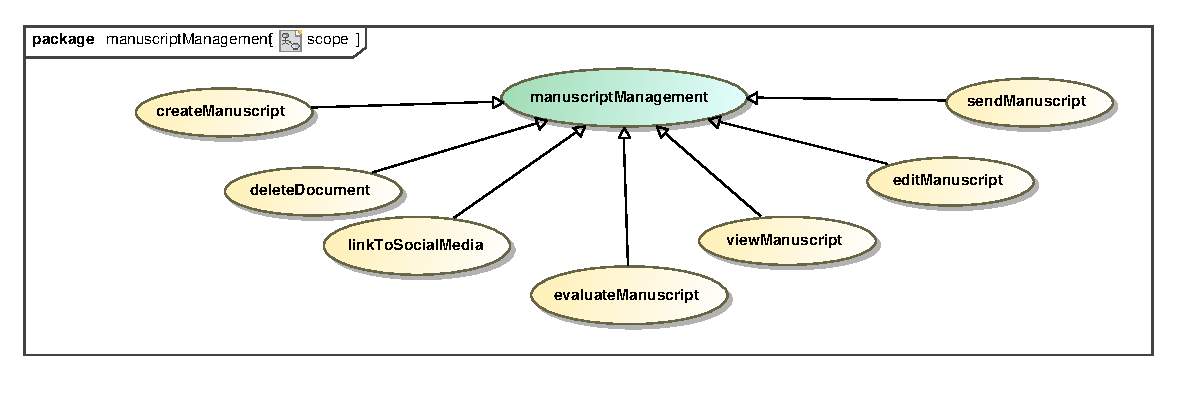
\includegraphics[height=200px, width=500px]{epsImages/ManuscriptManagement/scope.eps}
	\caption{Scope for manuscript management module}
\end{figure}

\newpage
\subsubsection{Use Cases}
\begin{enumerate}
\item \textbf{Create Manuscript - priority: critical}\\
\par{This use case creates a new project. It allows the user to give the manuscript a name and specify the privacy setting on it. }

\textbf{service contract:} below is a figure of the createManuscript service contract.

\begin{figure}[h]
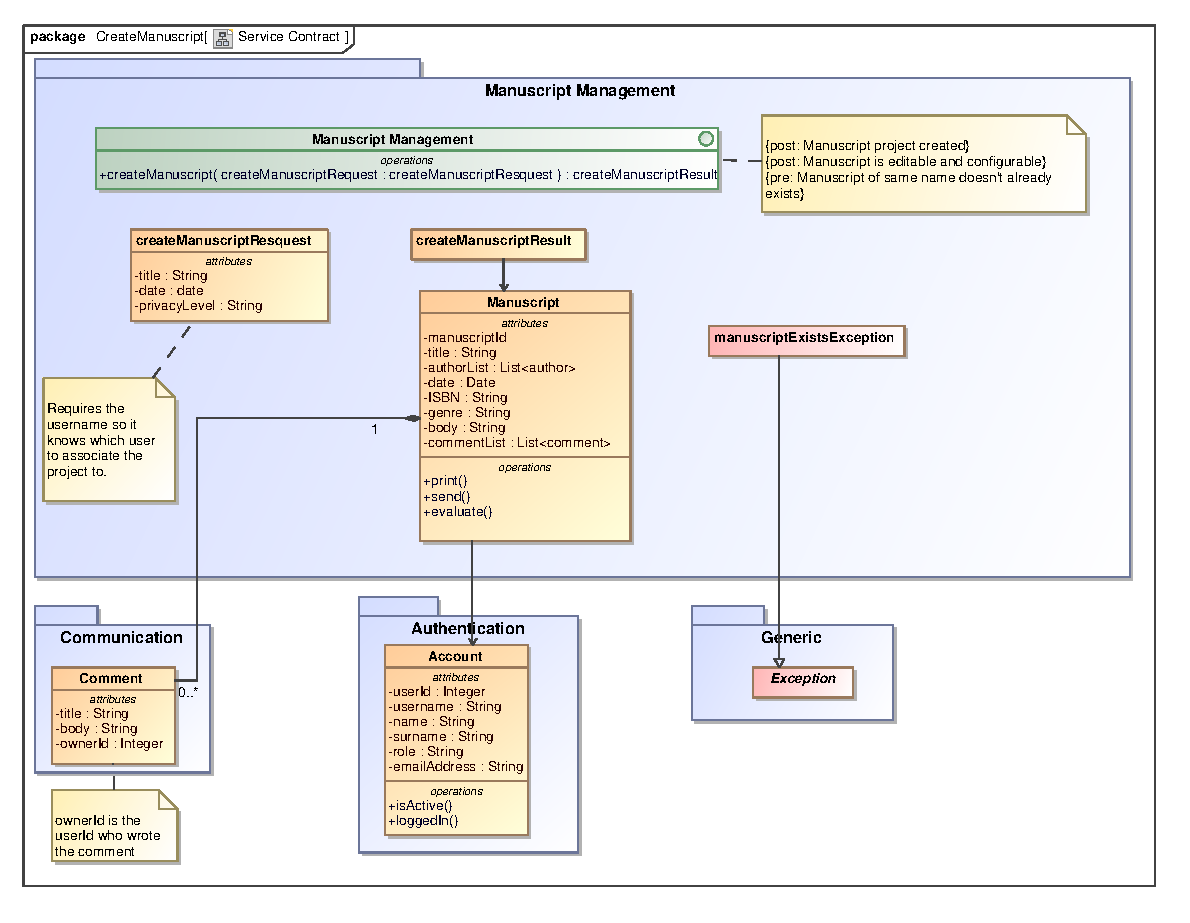
\includegraphics[height=300px, width=500px]{epsImages/ManuscriptManagement/createManuscriptServiceContract.eps}
\caption{Service contract for creating a new project (manuscript)}
\end{figure}


\item \textbf{deleteManuscript – priority: important}\\
\par{This use case which removes manuscript and persists changes to the database. }

\par{\textbf{service contract:} 
The service contract for the deleteManuscript  service is shown in figure below. The pre-conditions are enforced (raising the appropriate exception should they not be met) and the manuscript of interest is deleted and changes are persisted through to database.}

\begin{figure}[h]
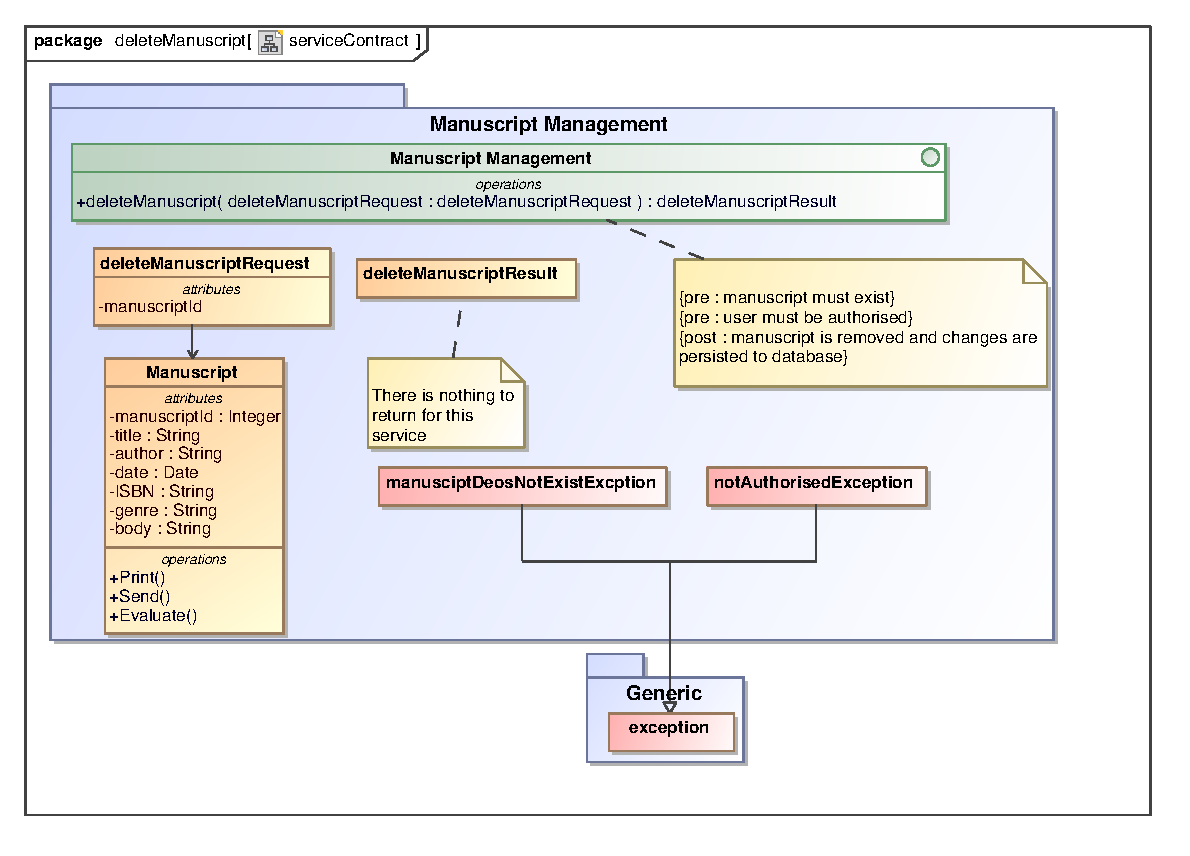
\includegraphics[height=300px, width=500px]{epsImages/ManuscriptManagement/deleteManuscript.eps}
\caption{Service contract for deleting a  project (manuscript)}
\end{figure}

\item \textbf{linkToSocialMedia – priority: important}\\
\par{important  This use case which link manuscript to social media and create an automated post}

\par{\textbf{service contract:} 
The service contract for the linkToSocialMedia service is shown in figure below. The pre-conditions are enforced (raising the appropriate exception should they not be met) and a post for the manuscript of interest  is created.}

\begin{figure}[h]
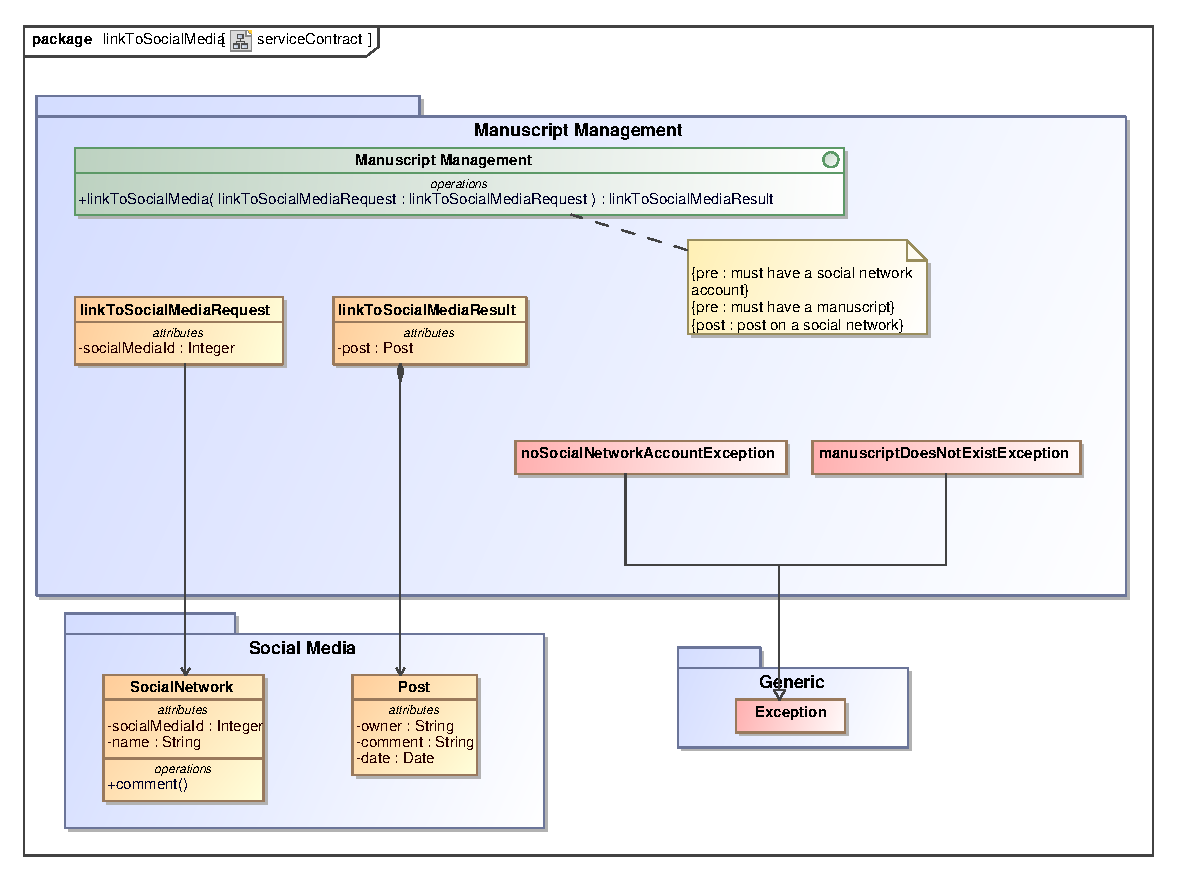
\includegraphics[height=300px, width=500px]{epsImages/ManuscriptManagement/linkToSocialMedia.eps}
\caption{Service contract for linking a  project (manuscript) to a social network}
\end{figure}


\item \textbf{editManuscript – priority: important}\\
\par{This use case which allows one to edit  manuscript and changes are persisted to database.}

\par{\textbf{service contract:} 
service contract The service contract for the editManuscript service is shown in figure below. The pre-conditions are enforced (raising the appropriate exception should they not be met) and the manuscript of interest is edited and changes are persisted to database}

\begin{figure}[h]
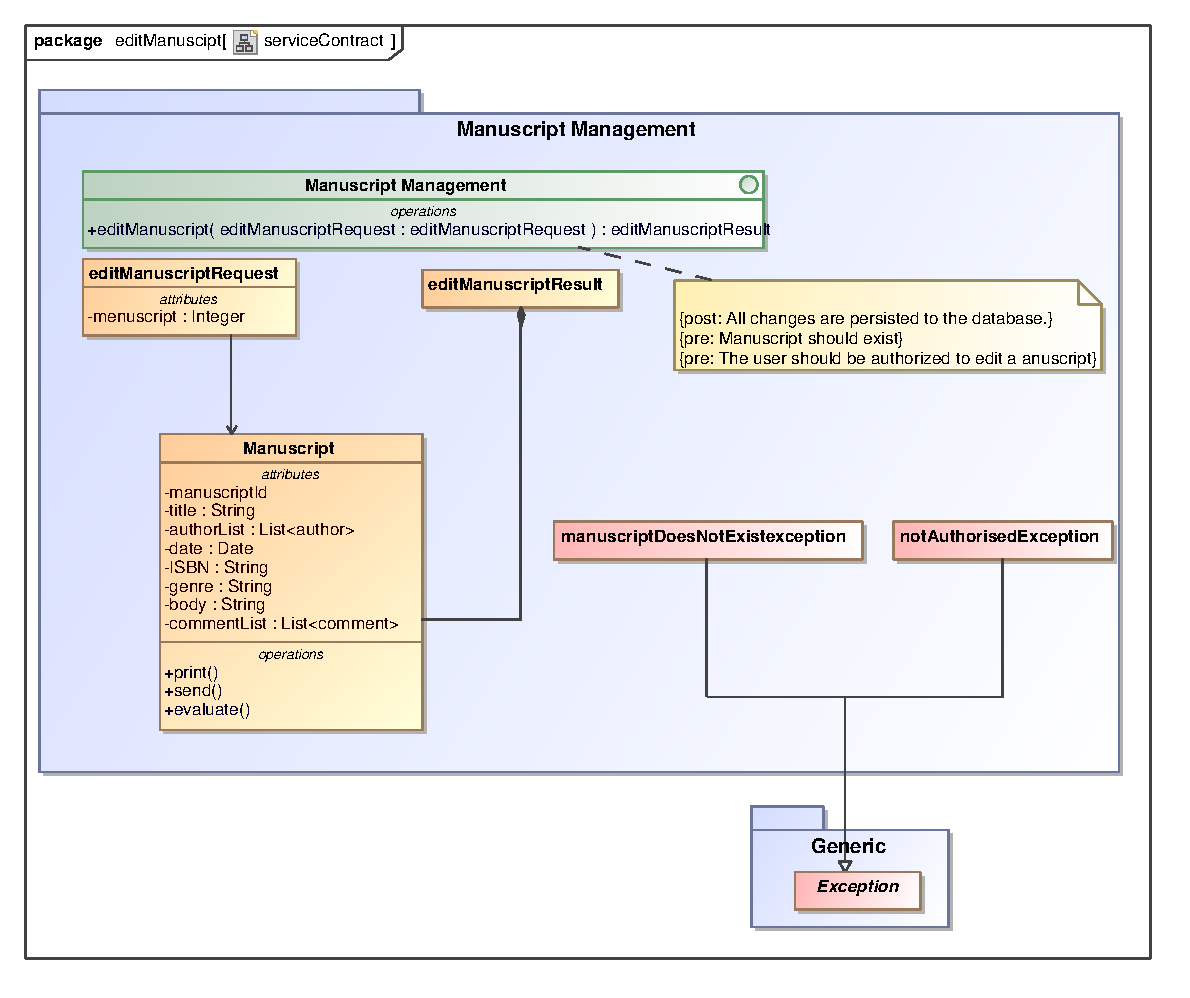
\includegraphics[height=250px, width=500px]{epsImages/ManuscriptManagement/editManuscript.eps}
\caption{Service contract for editing a  project (manuscript)}
\end{figure}
\newpage
\item \textbf{Evaluate Manuscript - priority: critical}
\par{This use case allows an agent or an editorial to evaluate the manuscript and to give the according feedback to the author, such as a comment or editorial letter.}

\begin{figure}[h]
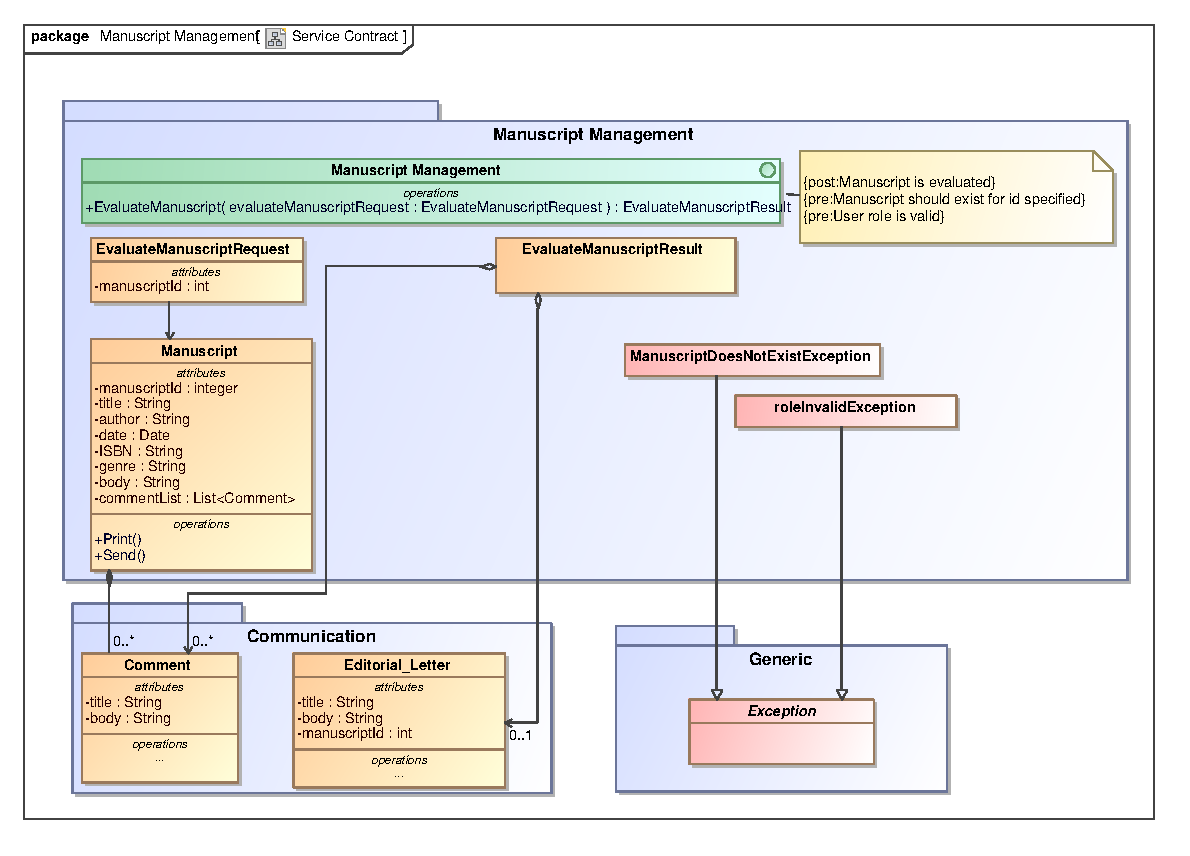
\includegraphics[height=300px, width=500px]{epsImages/ManuscriptManagement/EvaluateManuscript.eps}
\caption{Service contract for evaluating a manuscript}
\end{figure}

\item \textbf{Read Manuscript - priority: critical}
\par{This use case grants access to users to view/read the manuscript}

\begin{figure}[h]
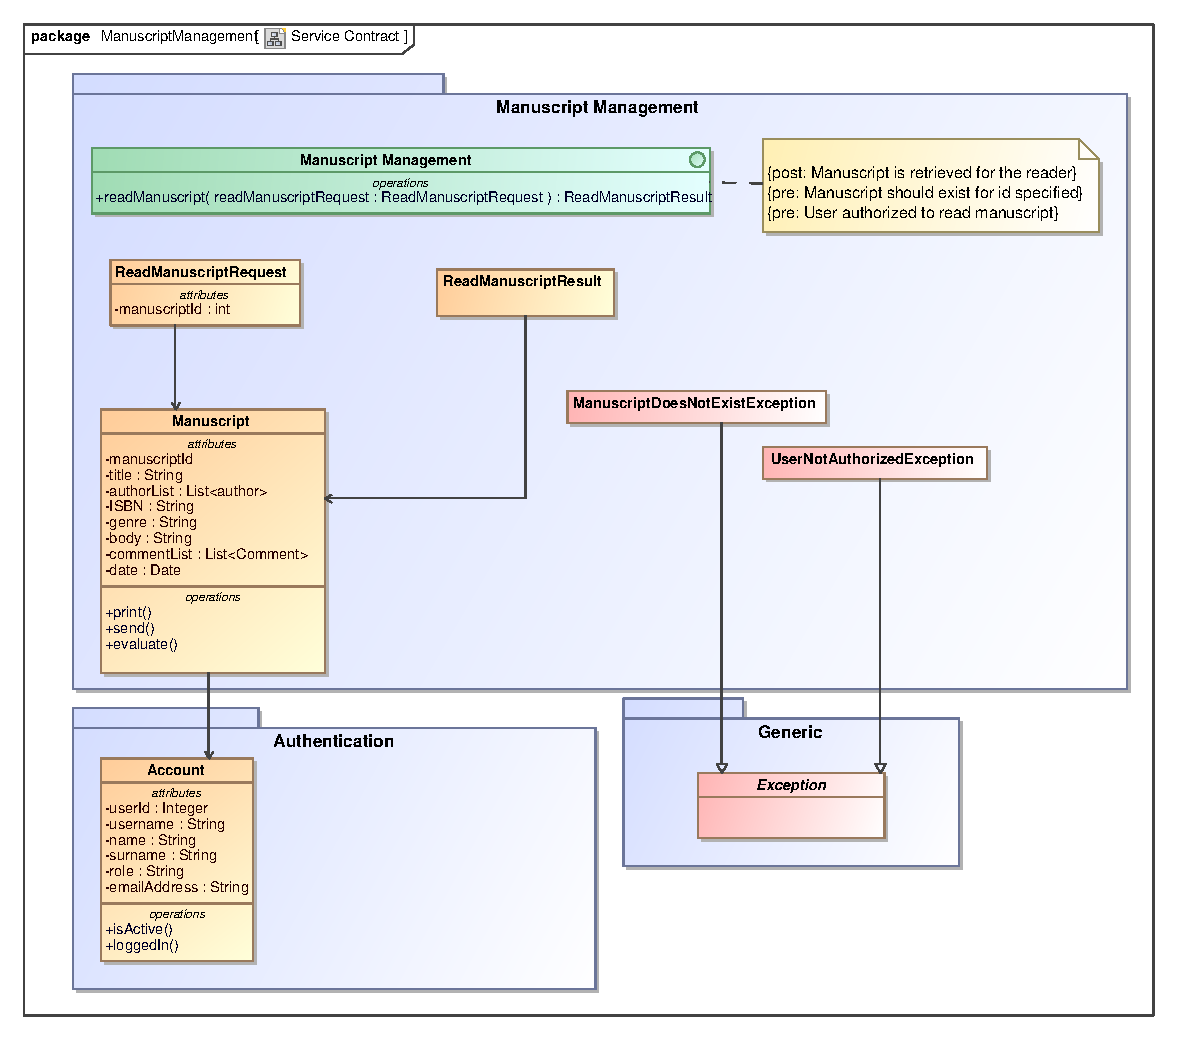
\includegraphics[height=300px, width=500px]{epsImages/ManuscriptManagement/ReadManuscript.eps}
\caption{Service contract for reading a manuscript}
\end{figure}

\item \textbf{Send Manuscript - priority: critical}\\
This use case allows a user link another user on the system to the manuscript. This allows the recipient to access it and, depending on the privileges afforded by the owner of the manuscript, be able to read/modify it.

\textbf{service contract:} below is a figure of the sendManuscript service contract.

\begin{figure}[h]
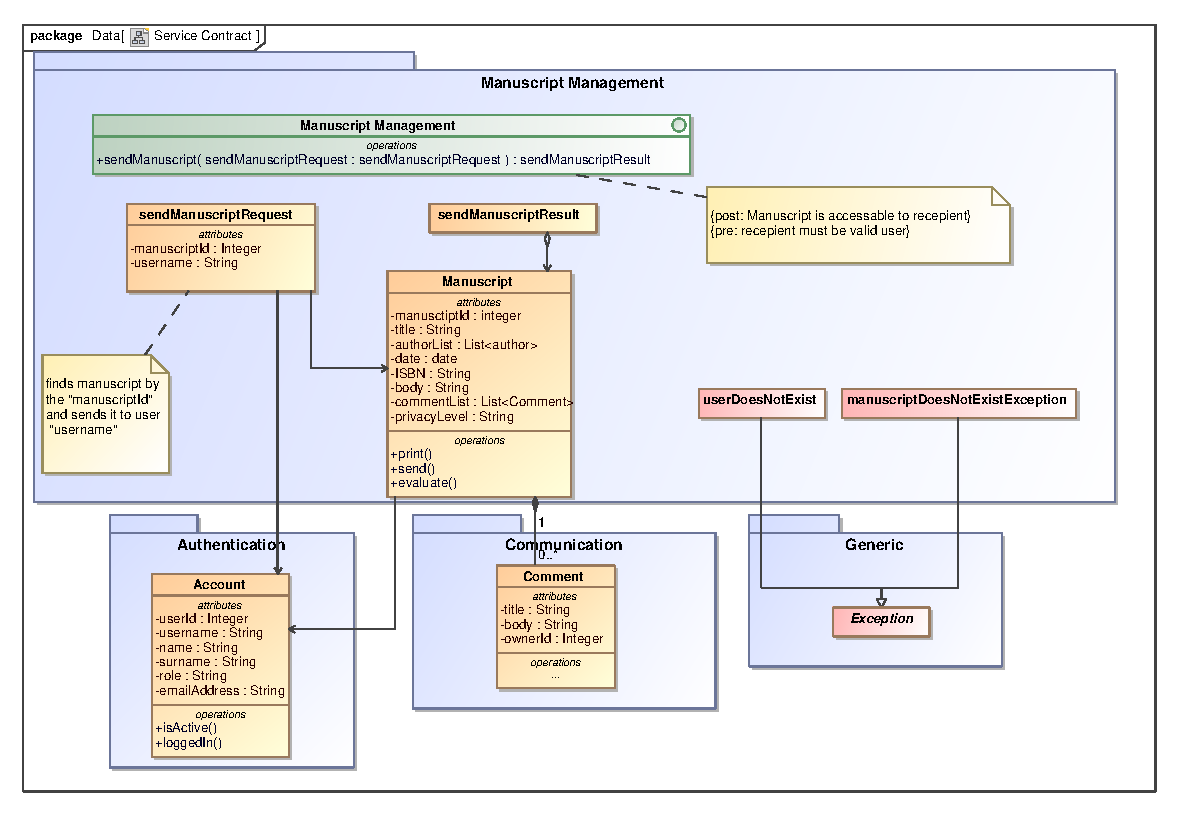
\includegraphics[height=250px, width=500px]{epsImages/ManuscriptManagement/sendManuscriptServiceContract.eps}
\caption{Service contract for sending a manuscript}
\end{figure}
 
\end{enumerate}

\subsection{Communication}

\begin{figure}[h]
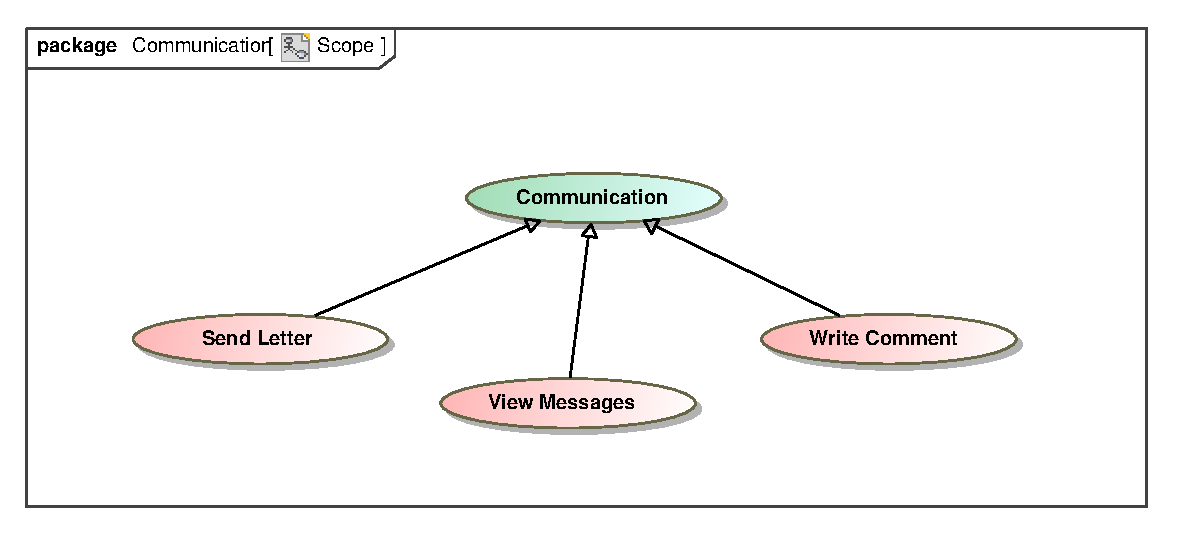
\includegraphics[height=250px, width=500px]{epsImages/Communication/CommunicationScope.eps}
\caption{Scope of Communication module}
\end{figure}

\subsubsection{scope}
\par{This section provides the details use case requirements for the use cases offered by the Authentication
module.}

\subsubsection{Use Cases}

\begin{enumerate}
\item \textbf{Send Letter - priority: critical}
\par{This use case allow the writing and sending of an appropriate letter to the corresponding user, such as a query letter to the agent. Available letters are: editorial letter, contract offer and query letter}

\begin{figure}[h]
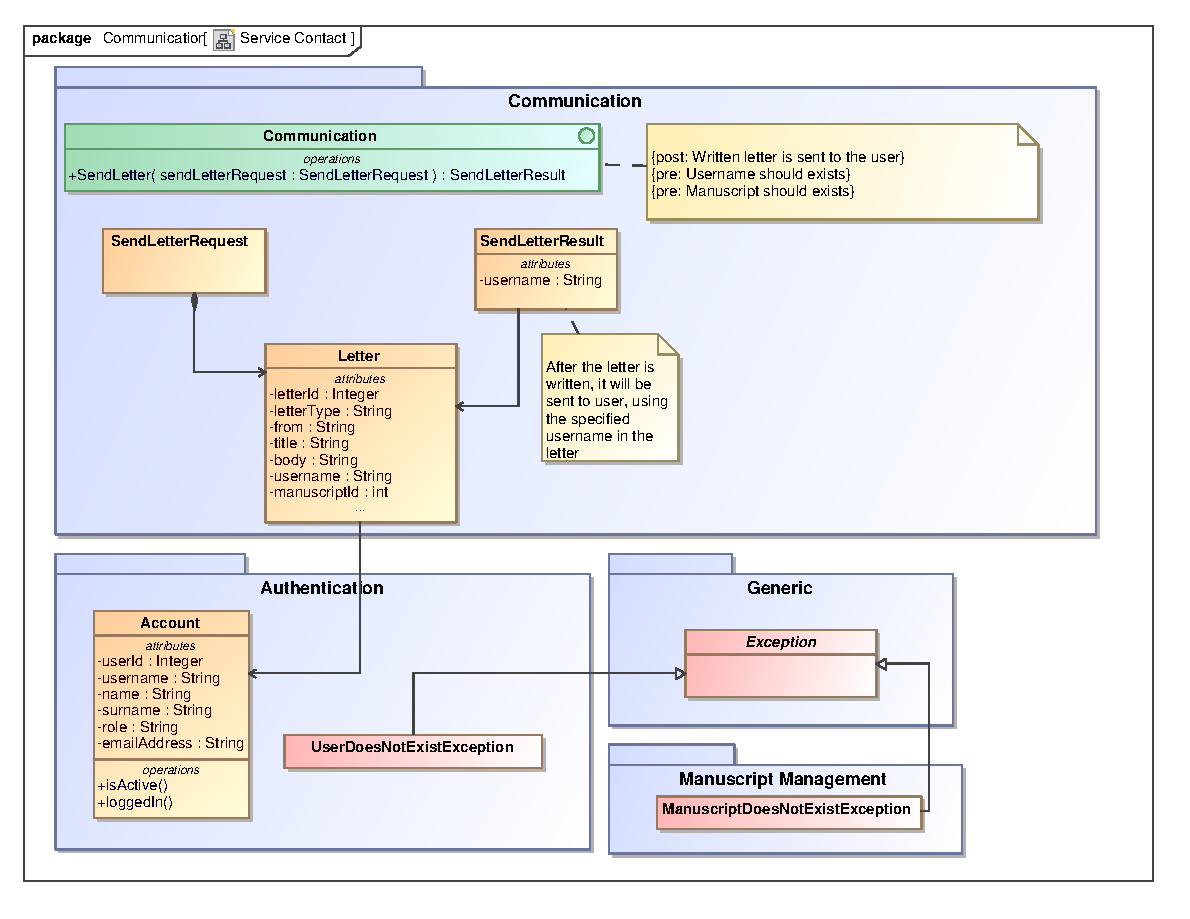
\includegraphics[height=250px, width=500px]{epsImages/Communication/sendLetterServiceContract.eps}
\caption{Service contract for sending a letter}
\end{figure}

\item \textbf{View Letter - priority: critical}\\
\par{This use case allows a user to view one of the letters sent to him/her. The letter can be an editorial letter, contract offer or query letter etc.}

\textbf{service contract:} Below is a diagram of a service contract of viewing a letter.

\begin{figure}[h]
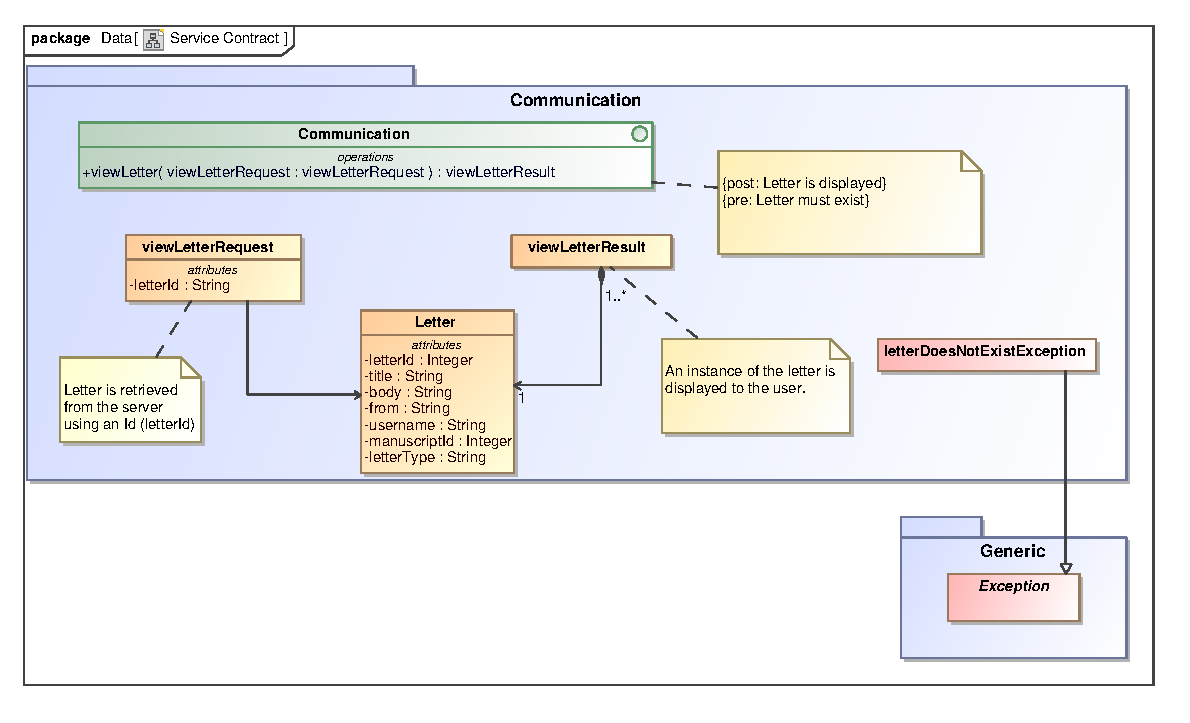
\includegraphics[height=250px, width=500px]{epsImages/Communication/viewLetterServiceContract.eps}
\caption{Service contract for viewing a letter}
\end{figure}
\newpage

\item \textbf{Write Comment}

\end{enumerate}

\subsection{Reporting}

\subsubsection{scope}
\par{This section provides the details use case requirements for the use cases offered by the Authentication
module.}

\begin{figure}[h]
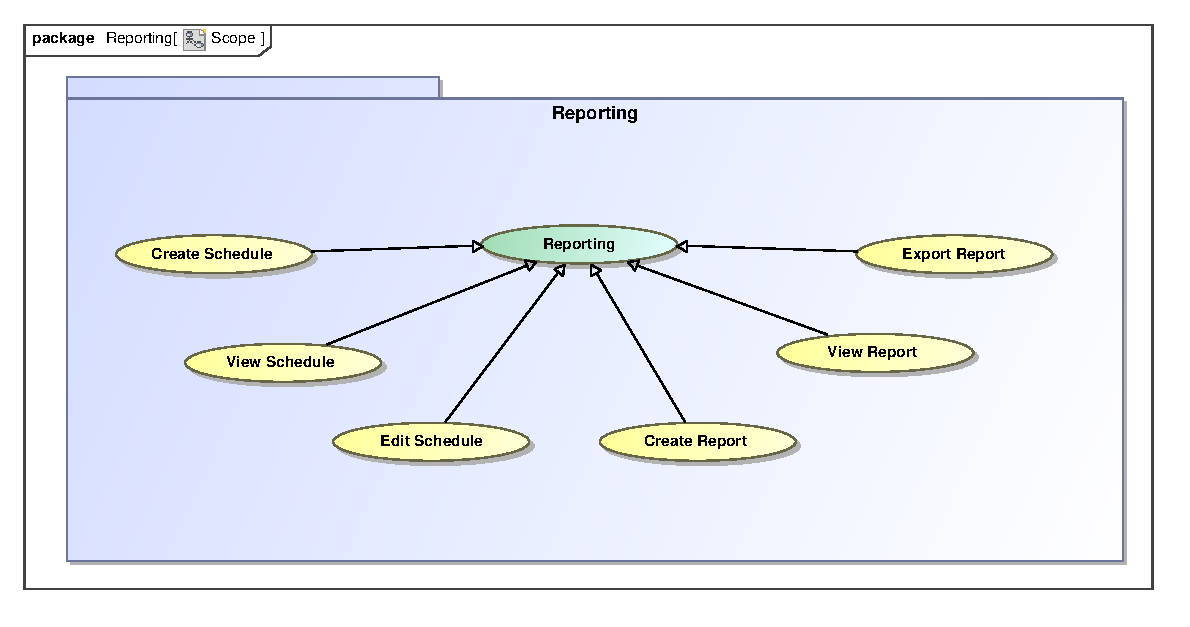
\includegraphics[height=250px, width=500px]{epsImages/Reporting/ReportScope.eps}
\caption{Scope of Reporting module}
\end{figure}


\subsubsection{Use Cases}

\begin{enumerate}
\item \textbf{CreateSchedule - priority: important}
\par{This use case allows a user to create a work schedule for the book that may consist of multiple tasks.}

\begin{figure}[h]
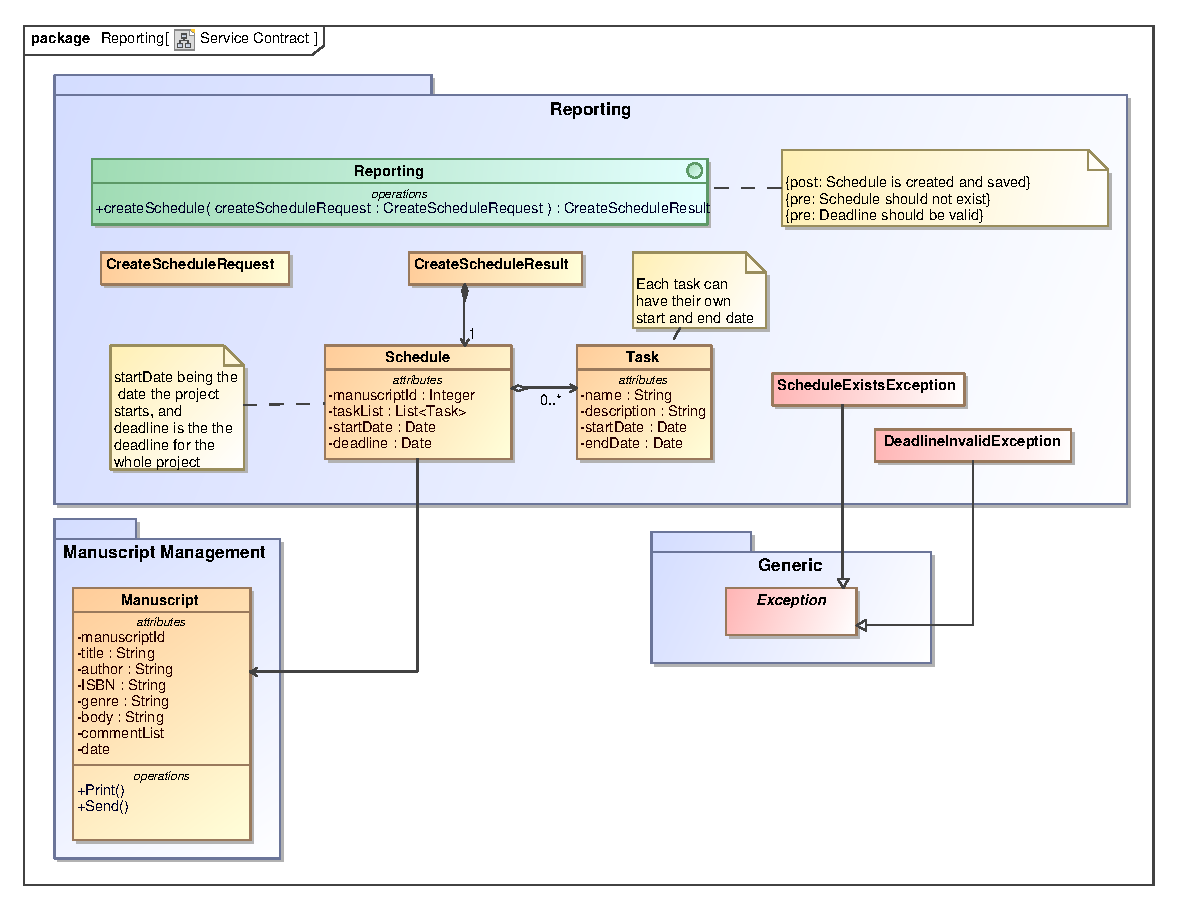
\includegraphics[height=250px, width=500px]{epsImages/Reporting/createSchedule.eps}
\caption{Service contract for creating a work schedule}
\end{figure}

\item \textbf{ViewSchedule - priority: important}
\par{This use case allows a user to view the work schedule for the book.}

\begin{figure}[h]
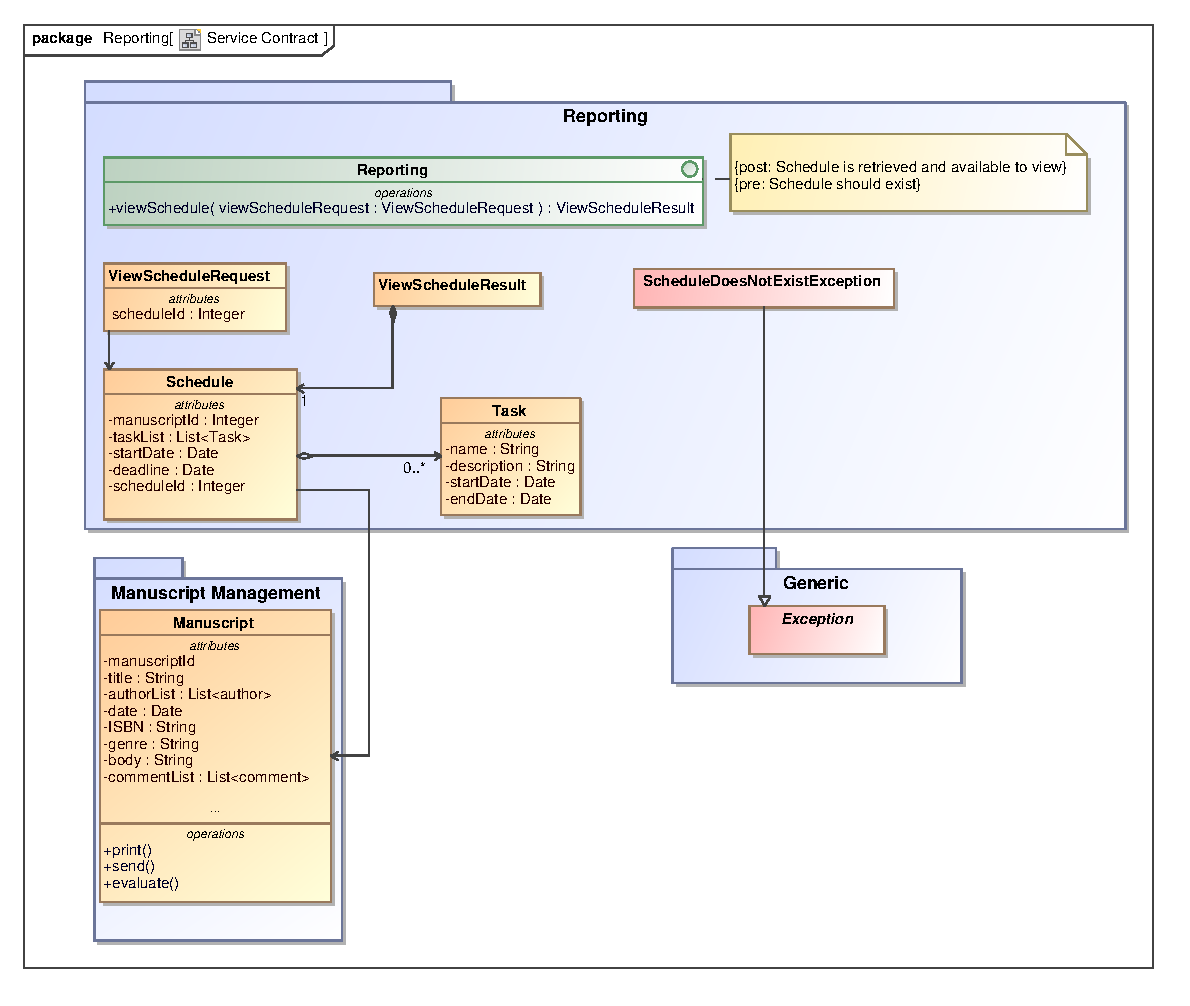
\includegraphics[height=250px, width=500px]{epsImages/Reporting/viewSchedule.eps}
\caption{Service contract for viewing a work schedule}
\end{figure}

\item \textbf{EditSchedule - priority: important}\\
\par{This use case allows a user to make changes to the work schedule of the book.}
\par{\textbf{service contract:} below is the service contract for editing a work schedule}

\begin{figure}[h]
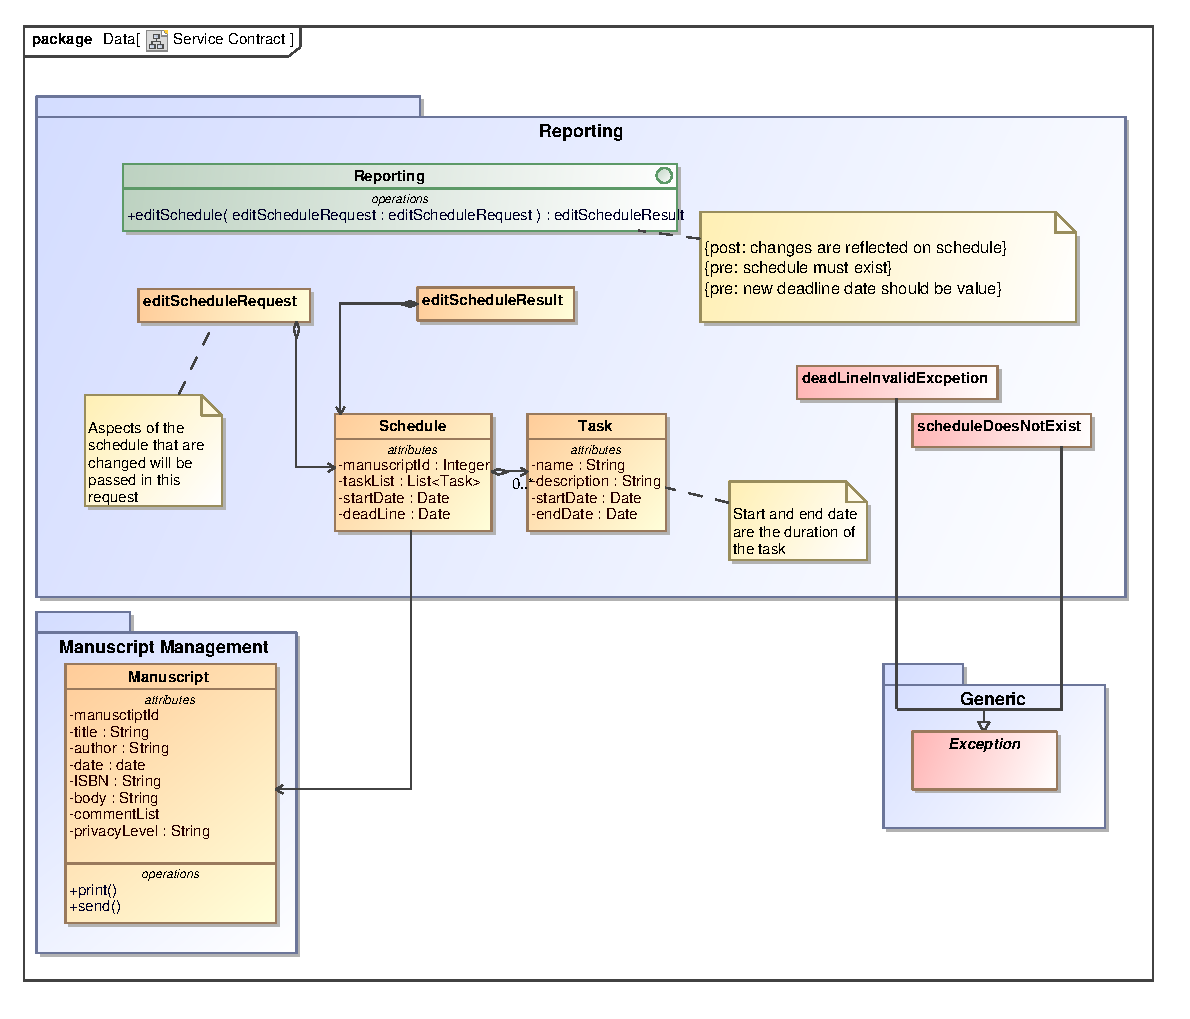
\includegraphics[height=250px, width=500px]{epsImages/Reporting/editScheduleServiceContract.eps}
\caption{Service contract for editing a work schedule}
\end{figure}

\item \textbf{createReport - priority: important}\\
\par{This use case creates  a report based on filters and provides it in printable format.}\\
\par{\textbf{service contract:} The service contract for the createReport  service is shown in figure below. The pre-conditions are enforced (raising the appropriate exception should they not be met) and the report is created and return in a printable format.}

\begin{figure}[h]
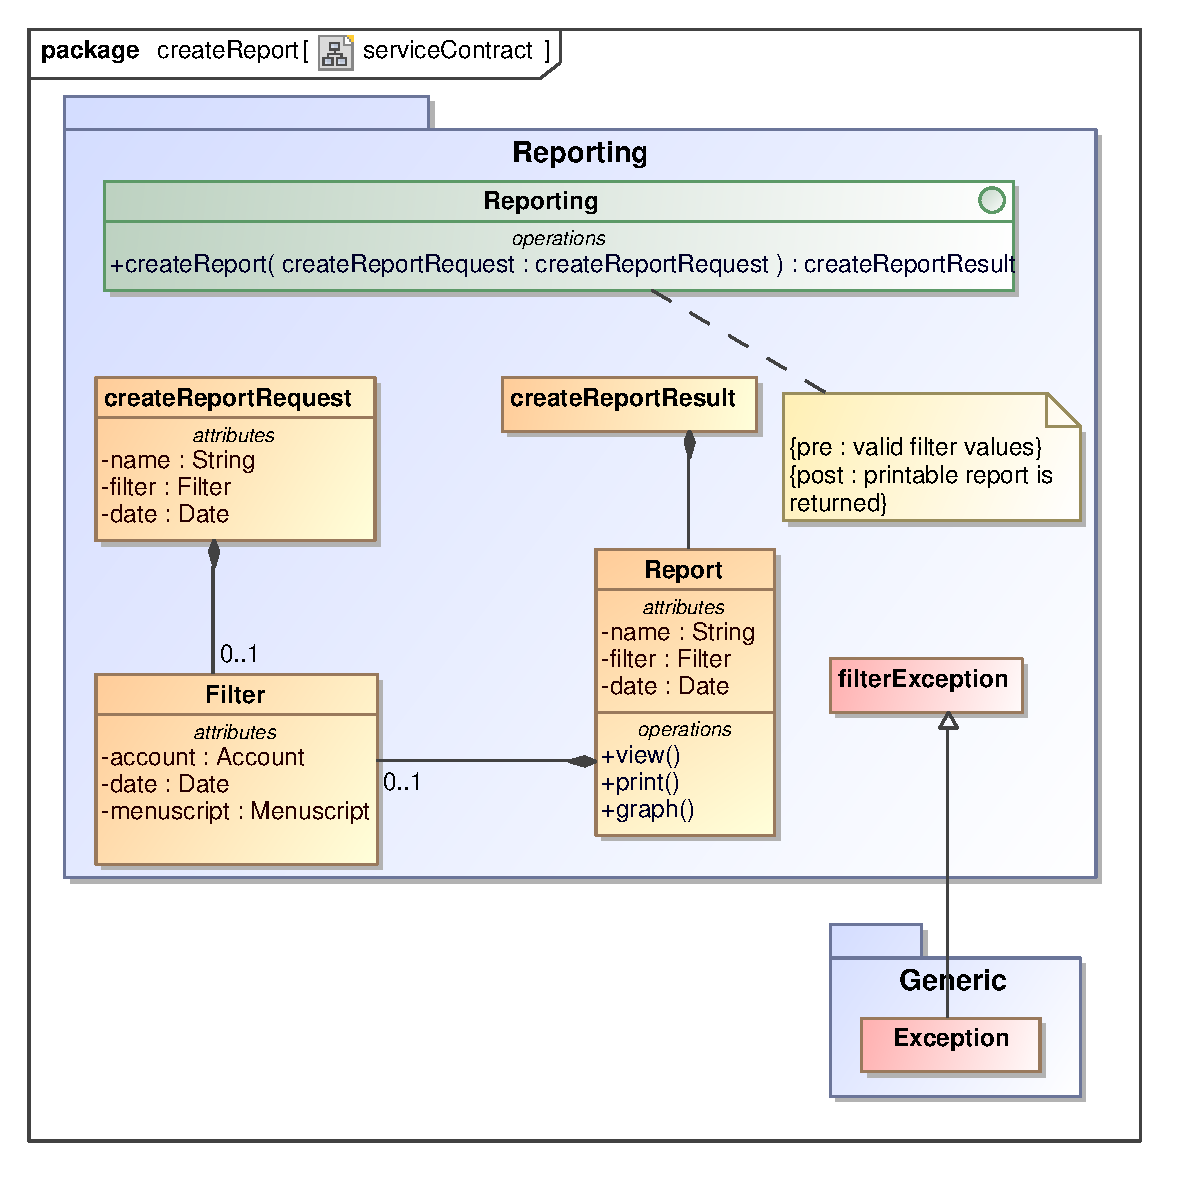
\includegraphics[height=250px, width=500px]{epsImages/Reporting/createReport.eps}
\caption{Service contract for creating a report}
\end{figure}

\item \textbf{viewReport - priority: important}\\
\par{This use case allows users to view a generated report, on the system (before exporting to say, a pdf for example).}\\
\par{\textbf{service contract:} Below is the service contract for viewing a report.}

\begin{figure}[h]
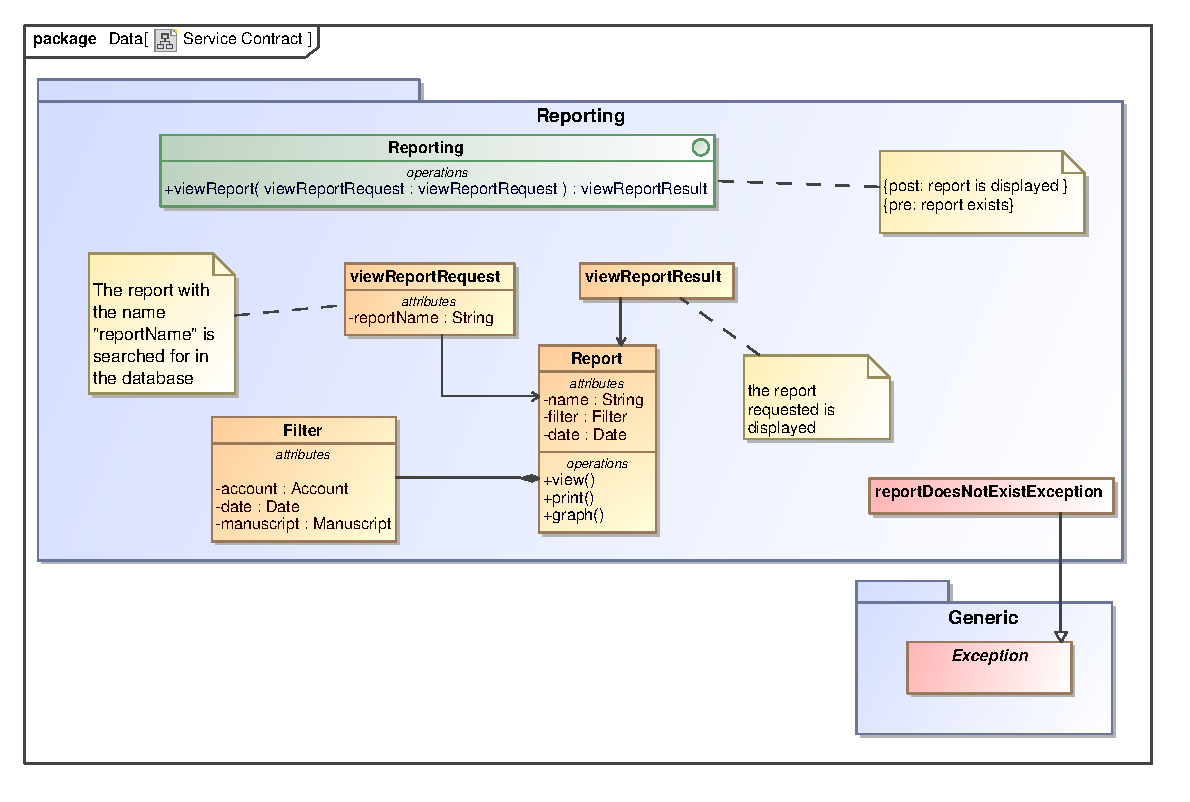
\includegraphics[height=250px, width=500px]{epsImages/Reporting/viewReportServiceContract.eps}
\caption{Service contract for viewing a report}
\end{figure}

 
\item \textbf{exportReport}
\par{priority: important  This use case which allows one to export a manuscript}\\
\par{\textbf{service contract:}} 

\begin{figure}[h]
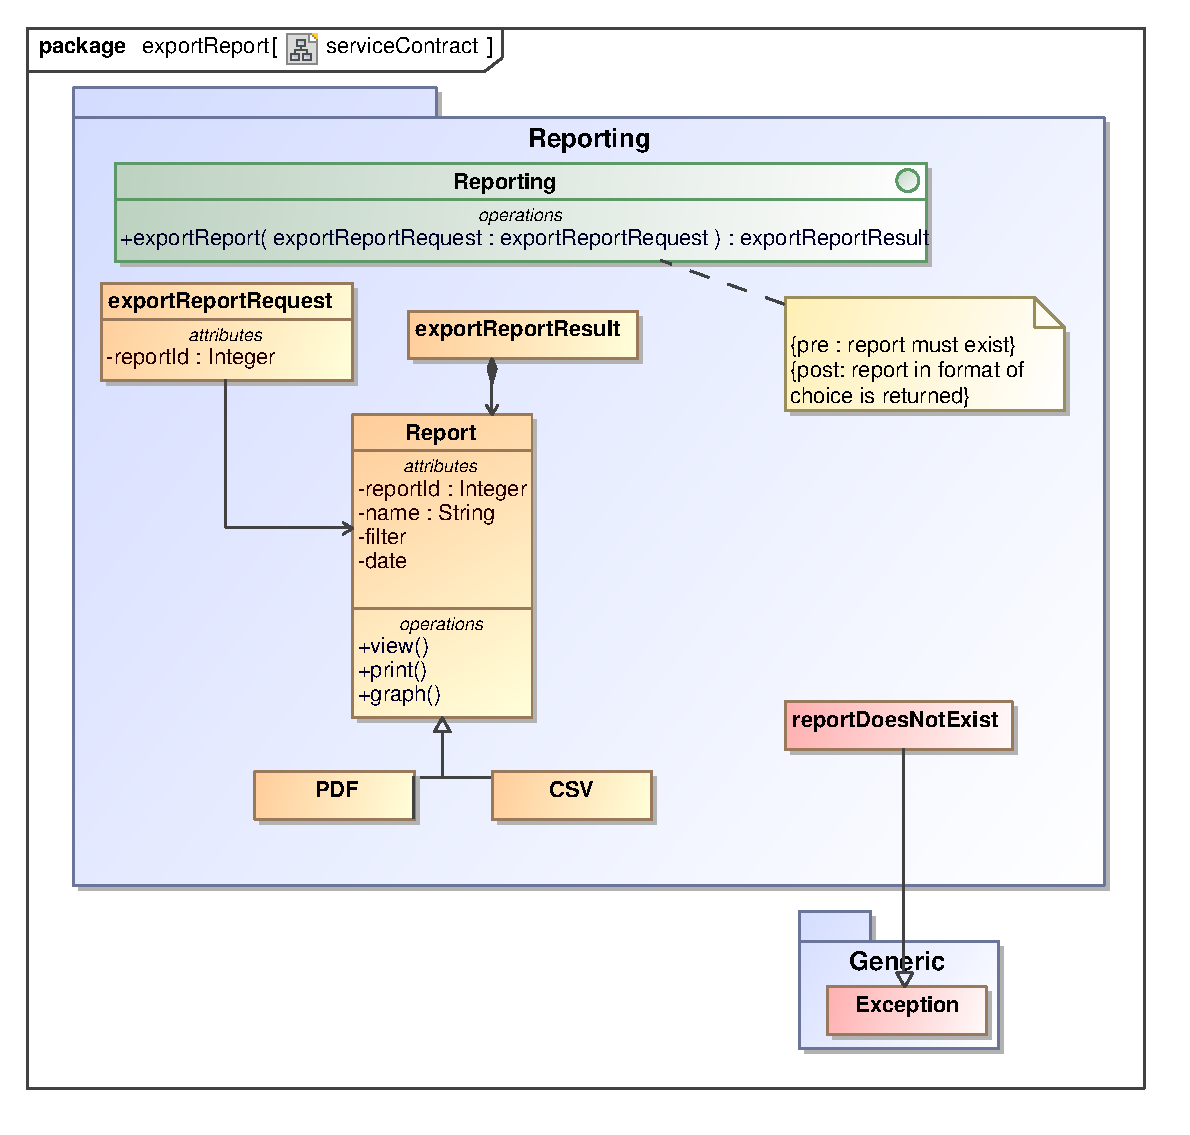
\includegraphics[height=250px, width=500px]{epsImages/Reporting/exportReport.eps}
\caption{Service contract for exporting a report}
\end{figure}
\end{enumerate}

\subsection{Design}

\subsubsection{scope}
\par{This section provides the details use case requirements for the use cases offered by the Authentication
module.}

\begin{figure}[h]
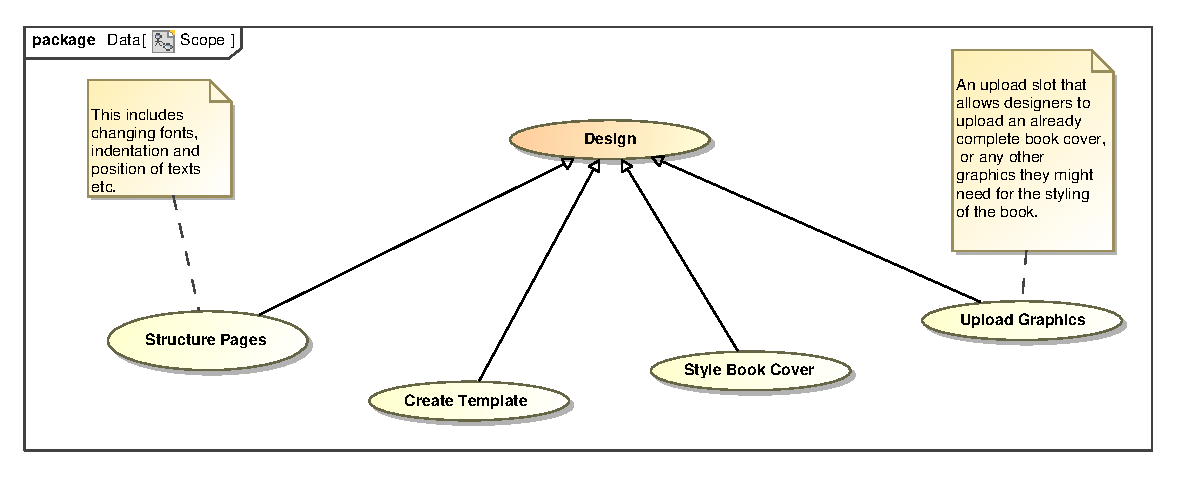
\includegraphics[height=250px, width=500px]{epsImages/Design/Scope.eps}
\caption{Scope of Design module}
\end{figure}

\subsubsection{Use Cases}
\begin{enumerate}
\item \textbf{structurePages - priority: critical}\\
\par{This use case which allows one to structure the  manuscript.}\\
\textbf{service contract:}

 \begin{figure}[h]
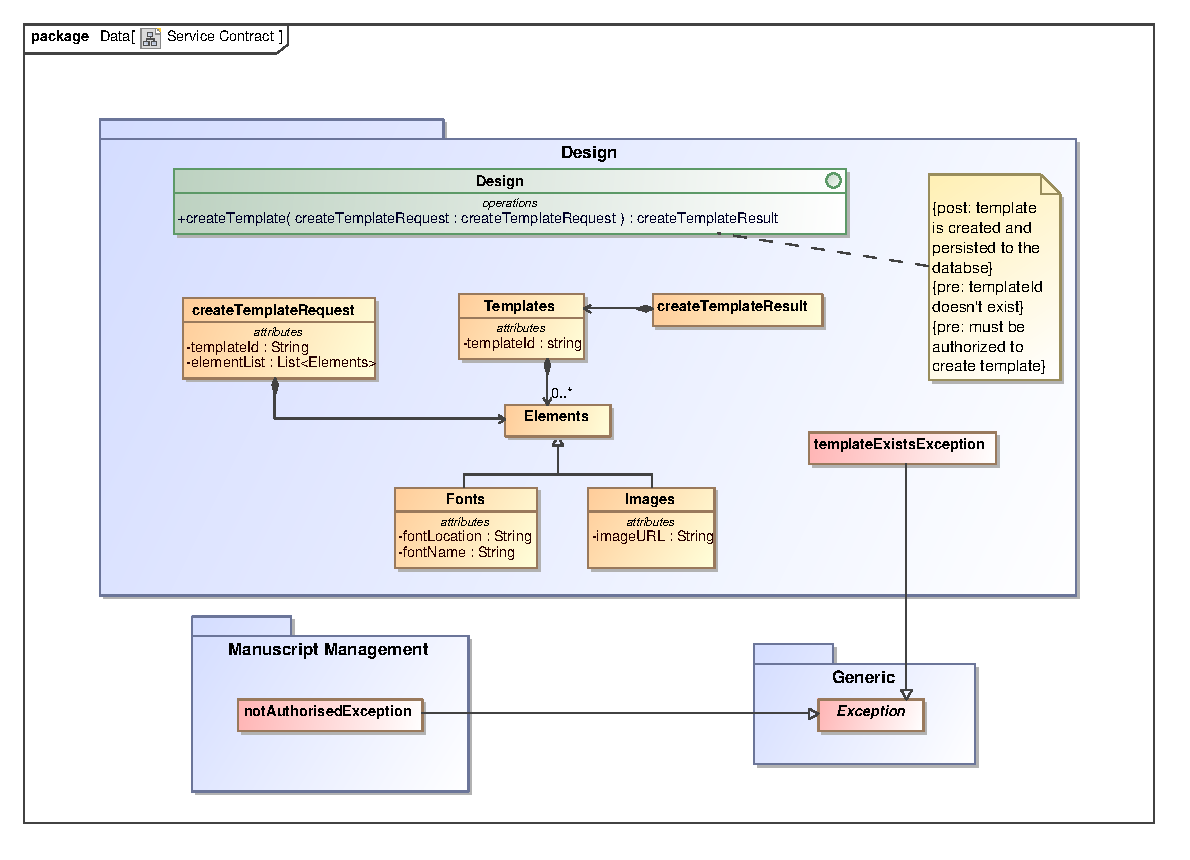
\includegraphics[height=250px, width=500px]{epsImages/Design/createTemplateServiceContract.eps}
\caption{Service contract for structuring a menuscript}
\end{figure}

\item \textbf{createTemplate - priority: nice to have}\\
\par{This module allows a user to create a template design for the book.}\\
\textbf{service contract:} Below is the service contract for creating a template.

 \begin{figure}[h]
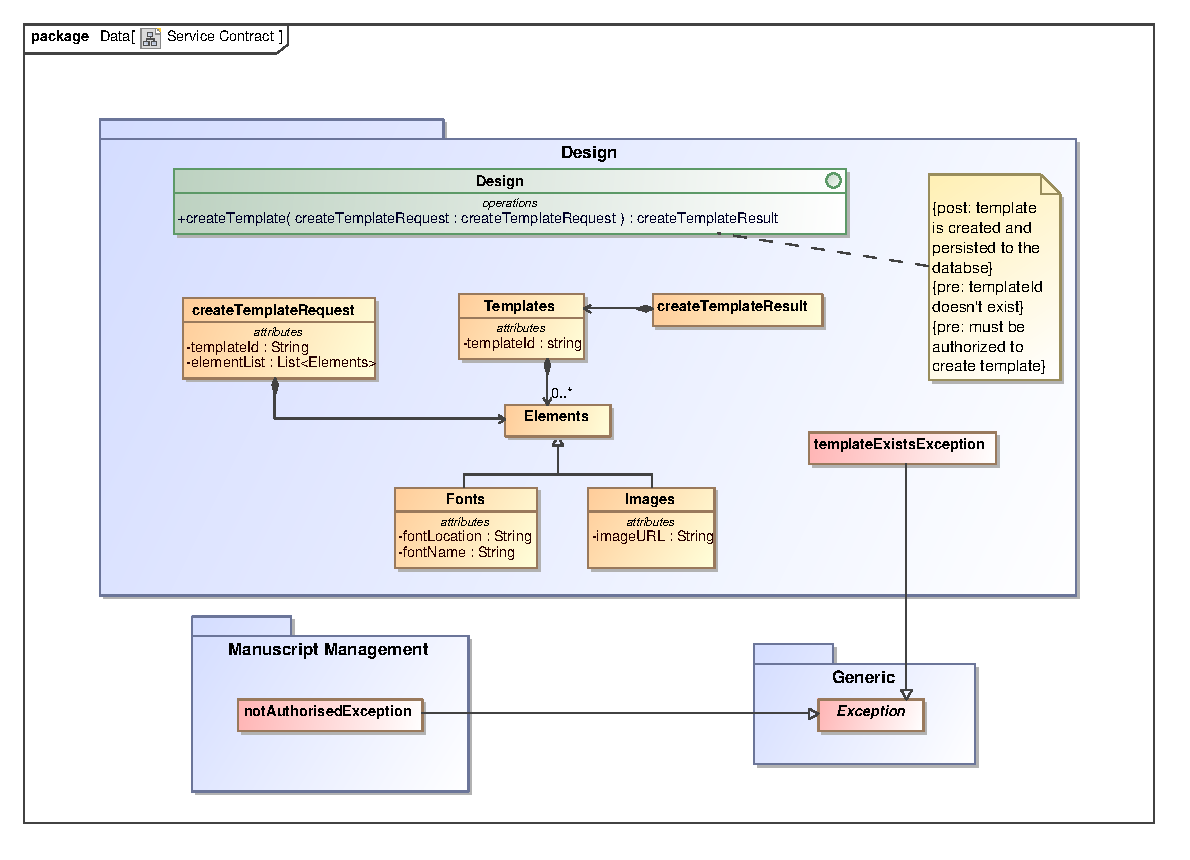
\includegraphics[height=250px, width=500px]{epsImages/Design/createTemplateServiceContract.eps}
\caption{Service contract for creating a template design}
\end{figure}

\item \textbf{createBookCover - priority: critical}
\par{This use case which allows create a book cover for a  manuscript.}\\
\textbf{service contract:}

 \begin{figure}[h]
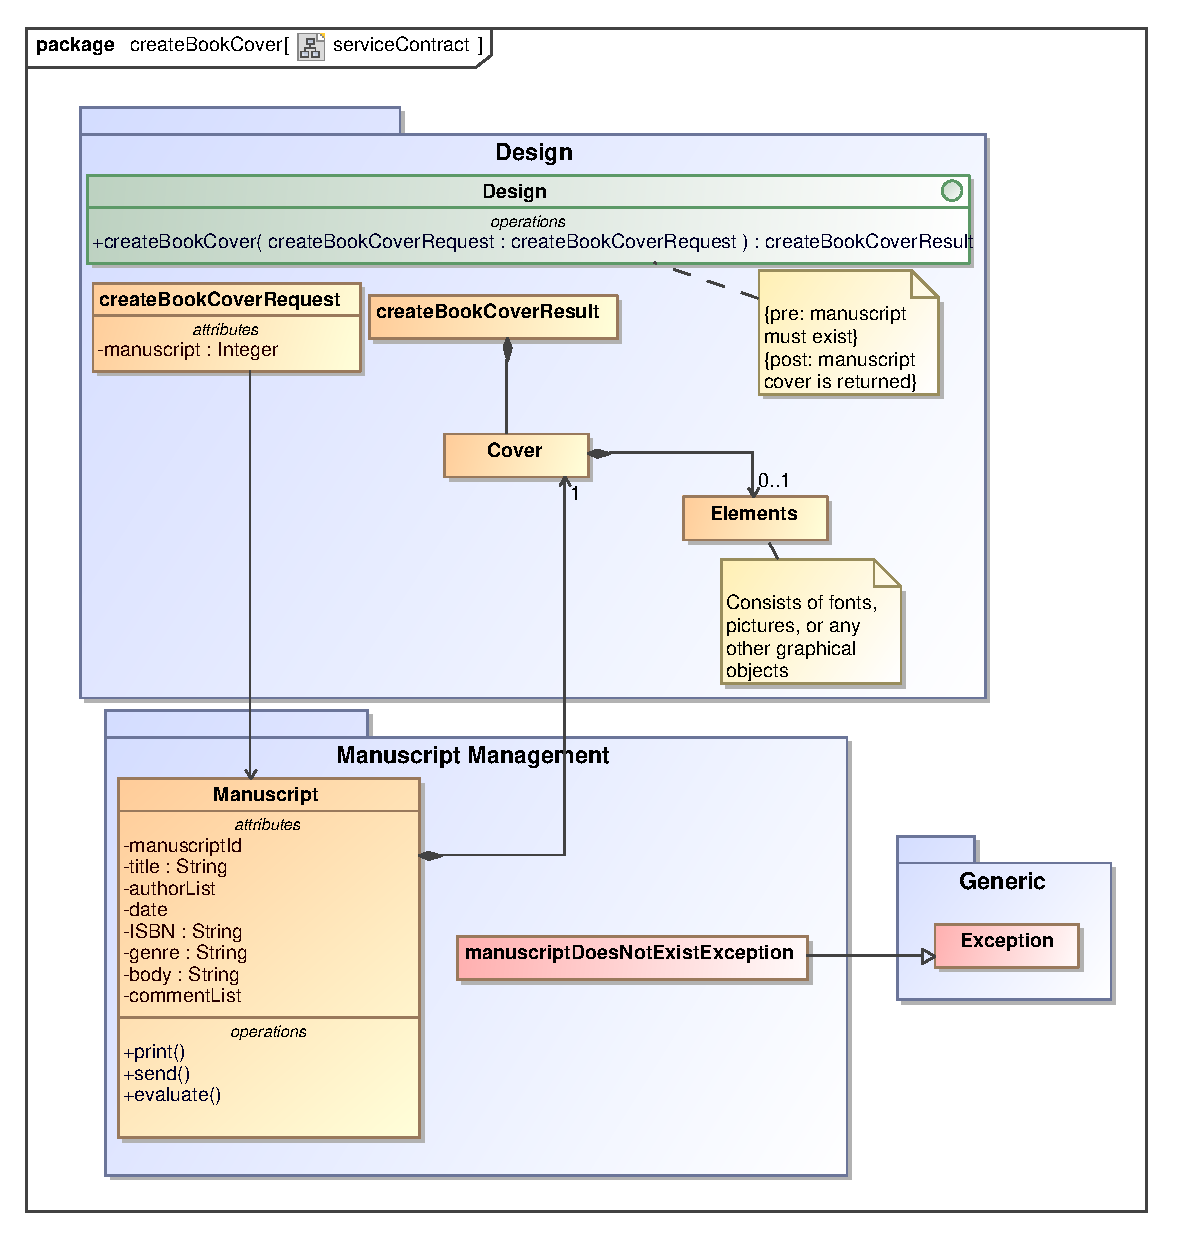
\includegraphics[height=250px, width=500px]{epsImages/Design/createBookCover.eps}
\caption{Service contract for creating a book cover}
\end{figure}
\item \textbf{uploadGraphic - priority: important}\\
\par{This use case allows a user to open any graphic they choose. This may be a new font, or image they wish to use, or a completed cover for the book. Size and format of a graphic are restricted however.}\\
\textbf{service contract:}Below is the service contract for uploading a graphic.

 \begin{figure}[h]
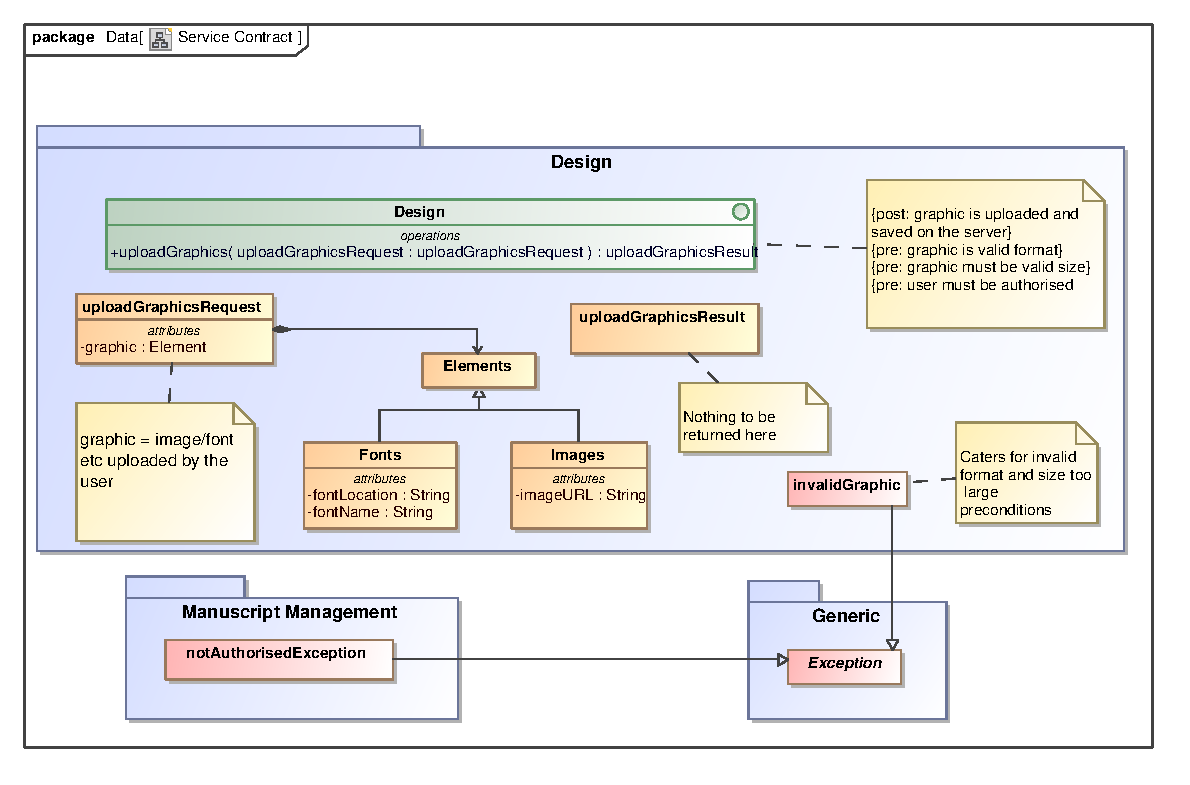
\includegraphics[height=250px, width=500px]{epsImages/Design/uploadGraphicsServiceContract.eps}
\caption{Service contract for uploading a graphic}
\end{figure}

\end{enumerate}
\end{document}
